\definecolor{a}{RGB}{235, 172, 35}
\definecolor{b}{RGB}{184, 0, 88}
\definecolor{c}{RGB}{0, 140, 249}
\definecolor{d}{RGB}{0, 110, 0}
\definecolor{e}{RGB}{0, 187, 173}
\definecolor{f}{RGB}{209, 99, 230}
\definecolor{g}{RGB}{178, 69, 2}
\definecolor{h}{RGB}{255, 146, 135}
\definecolor{i}{RGB}{89, 84, 214}
\definecolor{j}{RGB}{135, 133, 0}
\definecolor{k}{RGB}{0, 198, 248}

% GNUPLOT: LaTeX picture with Postscript
\begingroup
  \makeatletter
  \providecommand\color[2][]{%
    \GenericError{(gnuplot) \space\space\space\@spaces}{%
      Package color not loaded in conjunction with
      terminal option `colourtext'%
    }{See the gnuplot documentation for explanation.%
    }{Either use 'blacktext' in gnuplot or load the package
      color.sty in LaTeX.}%
    \renewcommand\color[2][]{}%
  }%
  \providecommand\includegraphics[2][]{%
    \GenericError{(gnuplot) \space\space\space\@spaces}{%
      Package graphicx or graphics not loaded%
    }{See the gnuplot documentation for explanation.%
    }{The gnuplot epslatex terminal needs graphicx.sty or graphics.sty.}%
    \renewcommand\includegraphics[2][]{}%
  }%
  \providecommand\rotatebox[2]{#2}%
  \@ifundefined{ifGPcolor}{%
    \newif\ifGPcolor
    \GPcolorfalse
  }{}%
  \@ifundefined{ifGPblacktext}{%
    \newif\ifGPblacktext
    \GPblacktexttrue
  }{}%
  % define a \g@addto@macro without @ in the name:
  \let\gplgaddtomacro\g@addto@macro
  % define empty templates for all commands taking text:
  \gdef\gplfronttext{}%
  \gdef\gplfronttext{}%
  \makeatother
  \ifGPblacktext
    % no textcolor at all
    \def\colorrgb#1{}%
    \def\colorgray#1{}%
  \else
    % gray or color?
    \ifGPcolor
      \def\colorrgb#1{\color[rgb]{#1}}%
      \def\colorgray#1{\color[gray]{#1}}%
      \expandafter\def\csname LTw\endcsname{\color{white}}%
      \expandafter\def\csname LTb\endcsname{\color{black}}%
      \expandafter\def\csname LTa\endcsname{\color{black}}%
      \expandafter\def\csname LT0\endcsname{\color[rgb]{1,0,0}}%
      \expandafter\def\csname LT1\endcsname{\color[rgb]{0,1,0}}%
      \expandafter\def\csname LT2\endcsname{\color[rgb]{0,0,1}}%
      \expandafter\def\csname LT3\endcsname{\color[rgb]{1,0,1}}%
      \expandafter\def\csname LT4\endcsname{\color[rgb]{0,1,1}}%
      \expandafter\def\csname LT5\endcsname{\color[rgb]{1,1,0}}%
      \expandafter\def\csname LT6\endcsname{\color[rgb]{0,0,0}}%
      \expandafter\def\csname LT7\endcsname{\color[rgb]{1,0.3,0}}%
      \expandafter\def\csname LT8\endcsname{\color[rgb]{0.5,0.5,0.5}}%
    \else
      % gray
      \def\colorrgb#1{\color{black}}%
      \def\colorgray#1{\color[gray]{#1}}%
      \expandafter\def\csname LTw\endcsname{\color{white}}%
      \expandafter\def\csname LTb\endcsname{\color{black}}%
      \expandafter\def\csname LTa\endcsname{\color{black}}%
      \expandafter\def\csname LT0\endcsname{\color{black}}%
      \expandafter\def\csname LT1\endcsname{\color{black}}%
      \expandafter\def\csname LT2\endcsname{\color{black}}%
      \expandafter\def\csname LT3\endcsname{\color{black}}%
      \expandafter\def\csname LT4\endcsname{\color{black}}%
      \expandafter\def\csname LT5\endcsname{\color{black}}%
      \expandafter\def\csname LT6\endcsname{\color{black}}%
      \expandafter\def\csname LT7\endcsname{\color{black}}%
      \expandafter\def\csname LT8\endcsname{\color{black}}%
    \fi
  \fi
    \setlength{\unitlength}{0.0500bp}%
    \ifx\gptboxheight\undefined%
      \newlength{\gptboxheight}%
      \newlength{\gptboxwidth}%
      \newsavebox{\gptboxtext}%
    \fi%
    \setlength{\fboxrule}{0.5pt}%
    \setlength{\fboxsep}{1pt}%
\begin{picture}(9500.00,4000.00)%
    \gplgaddtomacro\gplfronttext{%
      \colorrgb{0.15,0.15,0.15}%
      \put(818,1879){\makebox(0,0)[r]{\strut{}\footnotesize 8}}%
      \colorrgb{0.15,0.15,0.15}%
      \put(818,2141){\makebox(0,0)[r]{\strut{}\footnotesize 10}}%
      \colorrgb{0.15,0.15,0.15}%
      \put(818,2403){\makebox(0,0)[r]{\strut{}\footnotesize 12}}%
      \colorrgb{0.15,0.15,0.15}%
      \put(818,2665){\makebox(0,0)[r]{\strut{}\footnotesize 14}}%
      \colorrgb{0.15,0.15,0.15}%
      \put(818,2927){\makebox(0,0)[r]{\strut{}\footnotesize 16}}%
      \colorrgb{0.15,0.15,0.15}%
      \put(818,3189){\makebox(0,0)[r]{\strut{}\footnotesize 18}}%
      \colorrgb{0.15,0.15,0.15}%
      \put(818,3451){\makebox(0,0)[r]{\strut{}\footnotesize 20}}%
      \colorrgb{0.15,0.15,0.15}%
      \put(1015,1463){\makebox(0,0){\strut{}\footnotesize 6}}%
      \colorrgb{0.15,0.15,0.15}%
      \put(1277,1463){\makebox(0,0){\strut{}\footnotesize 8}}%
      \colorrgb{0.15,0.15,0.15}%
      \put(1539,1463){\makebox(0,0){\strut{}\footnotesize 10}}%
      \colorrgb{0.15,0.15,0.15}%
      \put(1801,1463){\makebox(0,0){\strut{}\footnotesize 12}}%
      \colorrgb{0.15,0.15,0.15}%
      \put(2063,1463){\makebox(0,0){\strut{}\footnotesize 14}}%
      \colorrgb{0.15,0.15,0.15}%
      \put(2325,1463){\makebox(0,0){\strut{}\footnotesize 16}}%
      \colorrgb{0.15,0.15,0.15}%
      \put(2587,1463){\makebox(0,0){\strut{}\footnotesize 18}}%
      \colorrgb{0.15,0.15,0.15}%
      \put(2849,1463){\makebox(0,0){\strut{}\footnotesize 20}}%
    }%
    \gplgaddtomacro\gplfronttext{%
      \colorrgb{0.15,0.15,0.15}%
      \put(312,2632){\rotatebox{90}{\makebox(0,0){\strut{}$y$ [m]}}}%
      \colorrgb{0.15,0.15,0.15}%
      \put(1899,1133){\makebox(0,0){\strut{}$x$ [m]}}%
      \put(1699,600){\makebox(0,0){\strut{} \footnotesize $|\mathcal{H}_A| = 100$ υποθέσεις (1 υπ./1.0 m$^2$)}}%
      \put(1699,300){\makebox(0,0){\strut{} \footnotesize $5 \times \{\bm{p}_i\} = 55$ απόπειρες εκτίμησης}}%
    }%
    \gplgaddtomacro\gplfronttext{%
      \colorrgb{0.15,0.15,0.15}%
      \put(3668,2933){\makebox(0,0)[r]{\strut{}\scriptsize $0\%$}}%
      \colorrgb{0.15,0.15,0.15}%
      \put(3668,3066){\makebox(0,0)[r]{\strut{}\scriptsize $20\%$}}%
      \colorrgb{0.15,0.15,0.15}%
      \put(3668,3199){\makebox(0,0)[r]{\strut{}\scriptsize $40\%$}}%
      \colorrgb{0.15,0.15,0.15}%
      \put(3668,3333){\makebox(0,0)[r]{\strut{}\scriptsize $60\%$}}%
      \colorrgb{0.15,0.15,0.15}%
      \put(3668,3466){\makebox(0,0)[r]{\strut{}\scriptsize $80\%$}}%
      \colorrgb{0.15,0.15,0.15}%
      \put(3668,3599){\makebox(0,0)[r]{\strut{}\scriptsize $100\%$}}%
      \colorrgb{0.15,0.15,0.15}%

    }%
    \gplgaddtomacro\gplfronttext{%
      \colorrgb{0.00,0.00,0.00}%
      \put(6000,3819){\makebox(0,0){\strut{}\footnotesize Ποσοστά αποτυχιών}}%
      \put(4700,4219){\makebox(0,0){\strut{}\footnotesize Μέσω \texttt{PLICP}}}%
      \put(7500,4219){\makebox(0,0){\strut{}\footnotesize Μέσω \texttt{FMI-SPOMF}}}%

    }%
    \gplgaddtomacro\gplfronttext{%
      \colorrgb{0.15,0.15,0.15}%
      \put(6518,2933){\makebox(0,0)[r]{\strut{}\scriptsize $0\%$}}%
      \colorrgb{0.15,0.15,0.15}%
      \put(6518,3066){\makebox(0,0)[r]{\strut{}\scriptsize $20\%$}}%
      \colorrgb{0.15,0.15,0.15}%
      \put(6518,3199){\makebox(0,0)[r]{\strut{}\scriptsize $40\%$}}%
      \colorrgb{0.15,0.15,0.15}%
      \put(6518,3333){\makebox(0,0)[r]{\strut{}\scriptsize $60\%$}}%
      \colorrgb{0.15,0.15,0.15}%
      \put(6518,3466){\makebox(0,0)[r]{\strut{}\scriptsize $80\%$}}%
      \colorrgb{0.15,0.15,0.15}%
      \put(6518,3599){\makebox(0,0)[r]{\strut{}\scriptsize $100\%$}}%
      \colorrgb{0.15,0.15,0.15}%

    }%
    \gplgaddtomacro\gplfronttext{%
    }%
    \gplgaddtomacro\gplfronttext{%
      \colorrgb{0.15,0.15,0.15}%
      \put(3668,1666){\makebox(0,0)[r]{\strut{}\scriptsize $0.0$}}%
      \colorrgb{0.15,0.15,0.15}%
      \put(3668,1833){\makebox(0,0)[r]{\strut{}\scriptsize $0.10$}}%
      \colorrgb{0.15,0.15,0.15}%
      \put(3668,1999){\makebox(0,0)[r]{\strut{}\scriptsize $0.20$}}%
      \colorrgb{0.15,0.15,0.15}%
      \put(3668,2166){\makebox(0,0)[r]{\strut{}\scriptsize $0.30$}}%
      \colorrgb{0.15,0.15,0.15}%
      \put(3668,2332){\makebox(0,0)[r]{\strut{}\scriptsize $0.40$}}%
      \colorrgb{0.15,0.15,0.15}%

    }%
    \gplgaddtomacro\gplfronttext{%
      \colorrgb{0.00,0.00,0.00}%
      \put(6000,2552){\makebox(0,0){\strut{}\footnotesize Μέσο σφάλμα στάσης [$(\text{m}^2 + \text{rad}^2)^{1/2}$]}}%
    }%
    \gplgaddtomacro\gplfronttext{%
      \colorrgb{0.15,0.15,0.15}%
      \put(6518,1666){\makebox(0,0)[r]{\strut{}\scriptsize $0.0$}}%
      \colorrgb{0.15,0.15,0.15}%
      \put(6518,1833){\makebox(0,0)[r]{\strut{}\scriptsize $0.10$}}%
      \colorrgb{0.15,0.15,0.15}%
      \put(6518,1999){\makebox(0,0)[r]{\strut{}\scriptsize $0.20$}}%
      \colorrgb{0.15,0.15,0.15}%
      \put(6518,2166){\makebox(0,0)[r]{\strut{}\scriptsize $0.30$}}%
      \colorrgb{0.15,0.15,0.15}%
      \put(6518,2332){\makebox(0,0)[r]{\strut{}\scriptsize $0.40$}}%
      \colorrgb{0.15,0.15,0.15}%

    }%
    \gplgaddtomacro\gplfronttext{%
    }%
    \gplgaddtomacro\gplfronttext{%
      \colorrgb{0.15,0.15,0.15}%
      \put(3668,400){\makebox(0,0)[r]{\strut{}\scriptsize $0$}}%
      \colorrgb{0.15,0.15,0.15}%
      %\put(3668,511){\makebox(0,0)[r]{\strut{}\scriptsize $200$}}%
      \colorrgb{0.15,0.15,0.15}%
      \put(3668,622){\makebox(0,0)[r]{\strut{}\scriptsize $400$}}%
      \colorrgb{0.15,0.15,0.15}%
      %\put(3668,733){\makebox(0,0)[r]{\strut{}\scriptsize $600$}}%
      \colorrgb{0.15,0.15,0.15}%
      \put(3668,844){\makebox(0,0)[r]{\strut{}\scriptsize $800$}}%
      \colorrgb{0.15,0.15,0.15}%
      %\put(3668,955){\makebox(0,0)[r]{\strut{}\scriptsize $1000$}}%
      \colorrgb{0.15,0.15,0.15}%
      \put(3668,1066){\makebox(0,0)[r]{\strut{}\scriptsize $1200$}}%
      \colorrgb{0.15,0.15,0.15}%
      \put(3958,180){\makebox(0,0){\strut{}\scriptsize \textcolor{a}{$\bm{p}_a^A$}}}%
      \colorrgb{0.15,0.15,0.15}%
      \put(4117,180){\makebox(0,0){\strut{}\scriptsize \textcolor{b}{$\bm{p}_b^A$}}}%
      \colorrgb{0.15,0.15,0.15}%
      \put(4275,180){\makebox(0,0){\strut{}\scriptsize \textcolor{c}{$\bm{p}_c^A$}}}%
      \colorrgb{0.15,0.15,0.15}%
      \put(4433,180){\makebox(0,0){\strut{}\scriptsize \textcolor{d}{$\bm{p}_d^A$}}}%
      \colorrgb{0.15,0.15,0.15}%
      \put(4591,180){\makebox(0,0){\strut{}\scriptsize \textcolor{e}{$\bm{p}_e^A$}}}%
      \colorrgb{0.15,0.15,0.15}%
      \put(4750,180){\makebox(0,0){\strut{}\scriptsize \textcolor{f}{$\bm{p}_f^A$}}}%
      \colorrgb{0.15,0.15,0.15}%
      \put(4908,180){\makebox(0,0){\strut{}\scriptsize \textcolor{g}{$\bm{p}_g^A$}}}%
      \colorrgb{0.15,0.15,0.15}%
      \put(5066,180){\makebox(0,0){\strut{}\scriptsize \textcolor{h}{$\bm{p}_h^A$}}}%
      \colorrgb{0.15,0.15,0.15}%
      \put(5224,180){\makebox(0,0){\strut{}\scriptsize \textcolor{i}{$\bm{p}_i^A$}}}%
      \colorrgb{0.15,0.15,0.15}%
      \put(5383,180){\makebox(0,0){\strut{}\scriptsize \textcolor{j}{$\bm{p}_j^A$}}}%
      \colorrgb{0.15,0.15,0.15}%
      \put(5541,180){\makebox(0,0){\strut{}\scriptsize \textcolor{k}{$\bm{p}_k^A$}}}%
    }%
    \gplgaddtomacro\gplfronttext{%
      \colorrgb{0.00,0.00,0.00}%
      \put(6000,1286){\makebox(0,0){\strut{}\footnotesize Μέσος χρόνος εκτέλεσης ανά υπόθεση [ms]}}%
    }%
    \gplgaddtomacro\gplfronttext{%
      \colorrgb{0.15,0.15,0.15}%
      \put(6518,400){\makebox(0,0)[r]{\strut{}\scriptsize $0$}}%
      \colorrgb{0.15,0.15,0.15}%
      %\put(6518,511){\makebox(0,0)[r]{\strut{}\scriptsize $200$}}%
      \colorrgb{0.15,0.15,0.15}%
      \put(6518,622){\makebox(0,0)[r]{\strut{}\scriptsize $400$}}%
      \colorrgb{0.15,0.15,0.15}%
      %\put(6518,733){\makebox(0,0)[r]{\strut{}\scriptsize $600$}}%
      \colorrgb{0.15,0.15,0.15}%
      \put(6518,844){\makebox(0,0)[r]{\strut{}\scriptsize $800$}}%
      \colorrgb{0.15,0.15,0.15}%
      %\put(6518,955){\makebox(0,0)[r]{\strut{}\scriptsize $1000$}}%
      \colorrgb{0.15,0.15,0.15}%
      \put(6518,1066){\makebox(0,0)[r]{\strut{}\scriptsize $1200$}}%
      \colorrgb{0.15,0.15,0.15}%
      \put(6808,180){\makebox(0,0){\strut{}\scriptsize \textcolor{a}{$\bm{p}_a^A$}}}%
      \colorrgb{0.15,0.15,0.15}%
      \put(6967,180){\makebox(0,0){\strut{}\scriptsize \textcolor{b}{$\bm{p}_b^A$}}}%
      \colorrgb{0.15,0.15,0.15}%
      \put(7125,180){\makebox(0,0){\strut{}\scriptsize \textcolor{c}{$\bm{p}_c^A$}}}%
      \colorrgb{0.15,0.15,0.15}%
      \put(7283,180){\makebox(0,0){\strut{}\scriptsize \textcolor{d}{$\bm{p}_d^A$}}}%
      \colorrgb{0.15,0.15,0.15}%
      \put(7441,180){\makebox(0,0){\strut{}\scriptsize \textcolor{e}{$\bm{p}_e^A$}}}%
      \colorrgb{0.15,0.15,0.15}%
      \put(7600,180){\makebox(0,0){\strut{}\scriptsize \textcolor{f}{$\bm{p}_f^A$}}}%
      \colorrgb{0.15,0.15,0.15}%
      \put(7758,180){\makebox(0,0){\strut{}\scriptsize \textcolor{g}{$\bm{p}_g^A$}}}%
      \colorrgb{0.15,0.15,0.15}%
      \put(7916,180){\makebox(0,0){\strut{}\scriptsize \textcolor{h}{$\bm{p}_h^A$}}}%
      \colorrgb{0.15,0.15,0.15}%
      \put(8074,180){\makebox(0,0){\strut{}\scriptsize \textcolor{i}{$\bm{p}_i^A$}}}%
      \colorrgb{0.15,0.15,0.15}%
      \put(8233,180){\makebox(0,0){\strut{}\scriptsize \textcolor{j}{$\bm{p}_j^A$}}}%
      \colorrgb{0.15,0.15,0.15}%
      \put(8391,180){\makebox(0,0){\strut{}\scriptsize \textcolor{k}{$\bm{p}_k^A$}}}%
    }%
    \gplgaddtomacro\gplfronttext{%
    }%
    \put(0,0){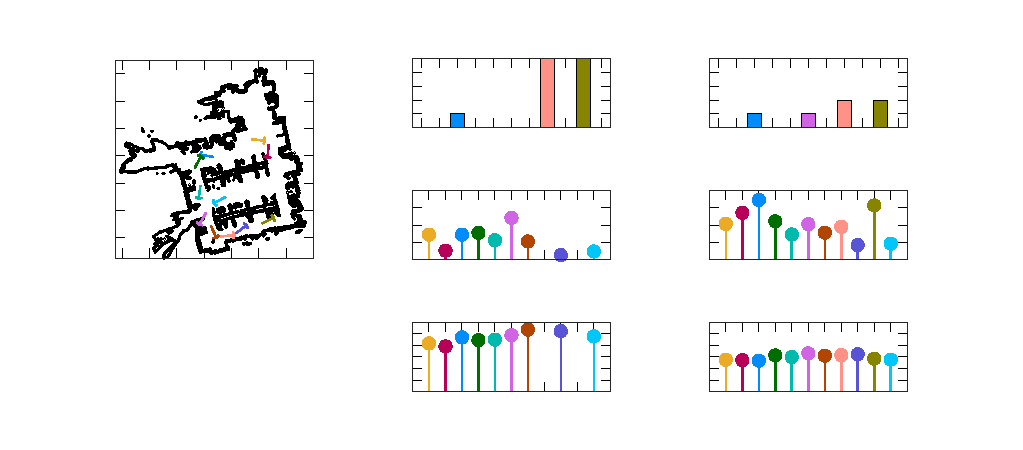
\includegraphics{./figures/slides/ch5/experiments//results_csal}}%
    \gplfronttext
  \end{picture}%
\endgroup
